%!TEX root = ../MasterThesis.tex

\section{Computer-Supported Cooperative Work}
\label{sec:cscw}

\subsection{Definition}
\label{sec:cscw_definition}

% section cscw_defintion (end)

\subsection{Types}
\label{sec:cscw_types}

CSCW systems can be differentiated by their support of communication on the two axis place and time: \\

\begin{figure}[H]
 \centering
 %\includesvg[width=0.8\columnwidth, svgpath = images/]{cscw_time_place_matrix}
 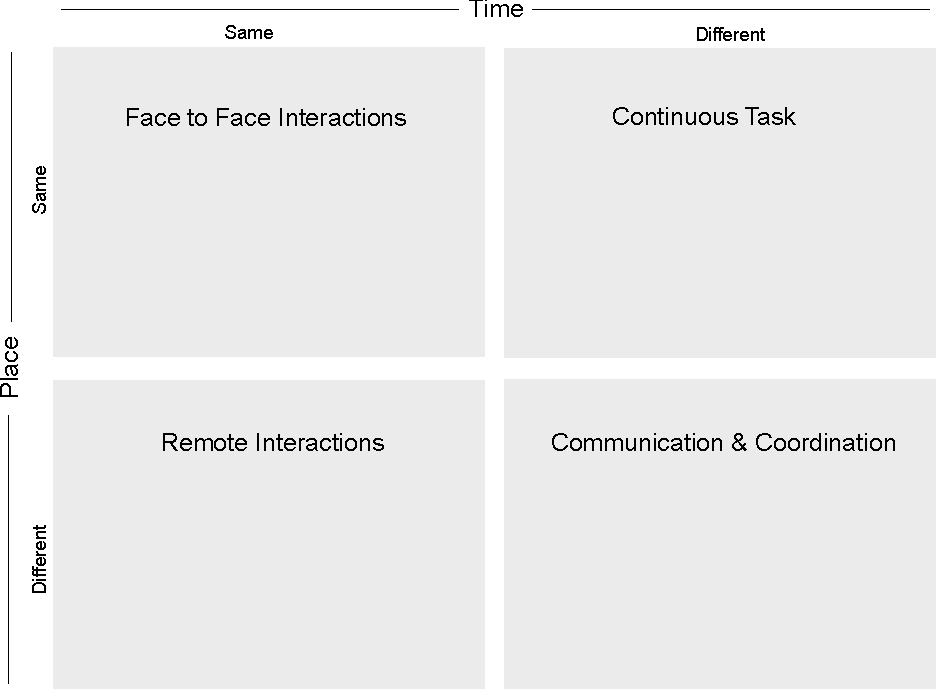
\includegraphics[width=0.8\columnwidth]{images/cscw_time_place_matrix.pdf}
 \caption{CSCW Place/Time Matrix \citep{xx}}
\label{fig:images_cscw_time_place_matrix}
\end{figure}

Additionally it is possible to group the CSCW systems based on the 3C model: \\

\begin{figure}[H]
 \centering
 %\includesvg[width=0.5\columnwidth, svgpath = images/]{cscw_time_place_matrix}
 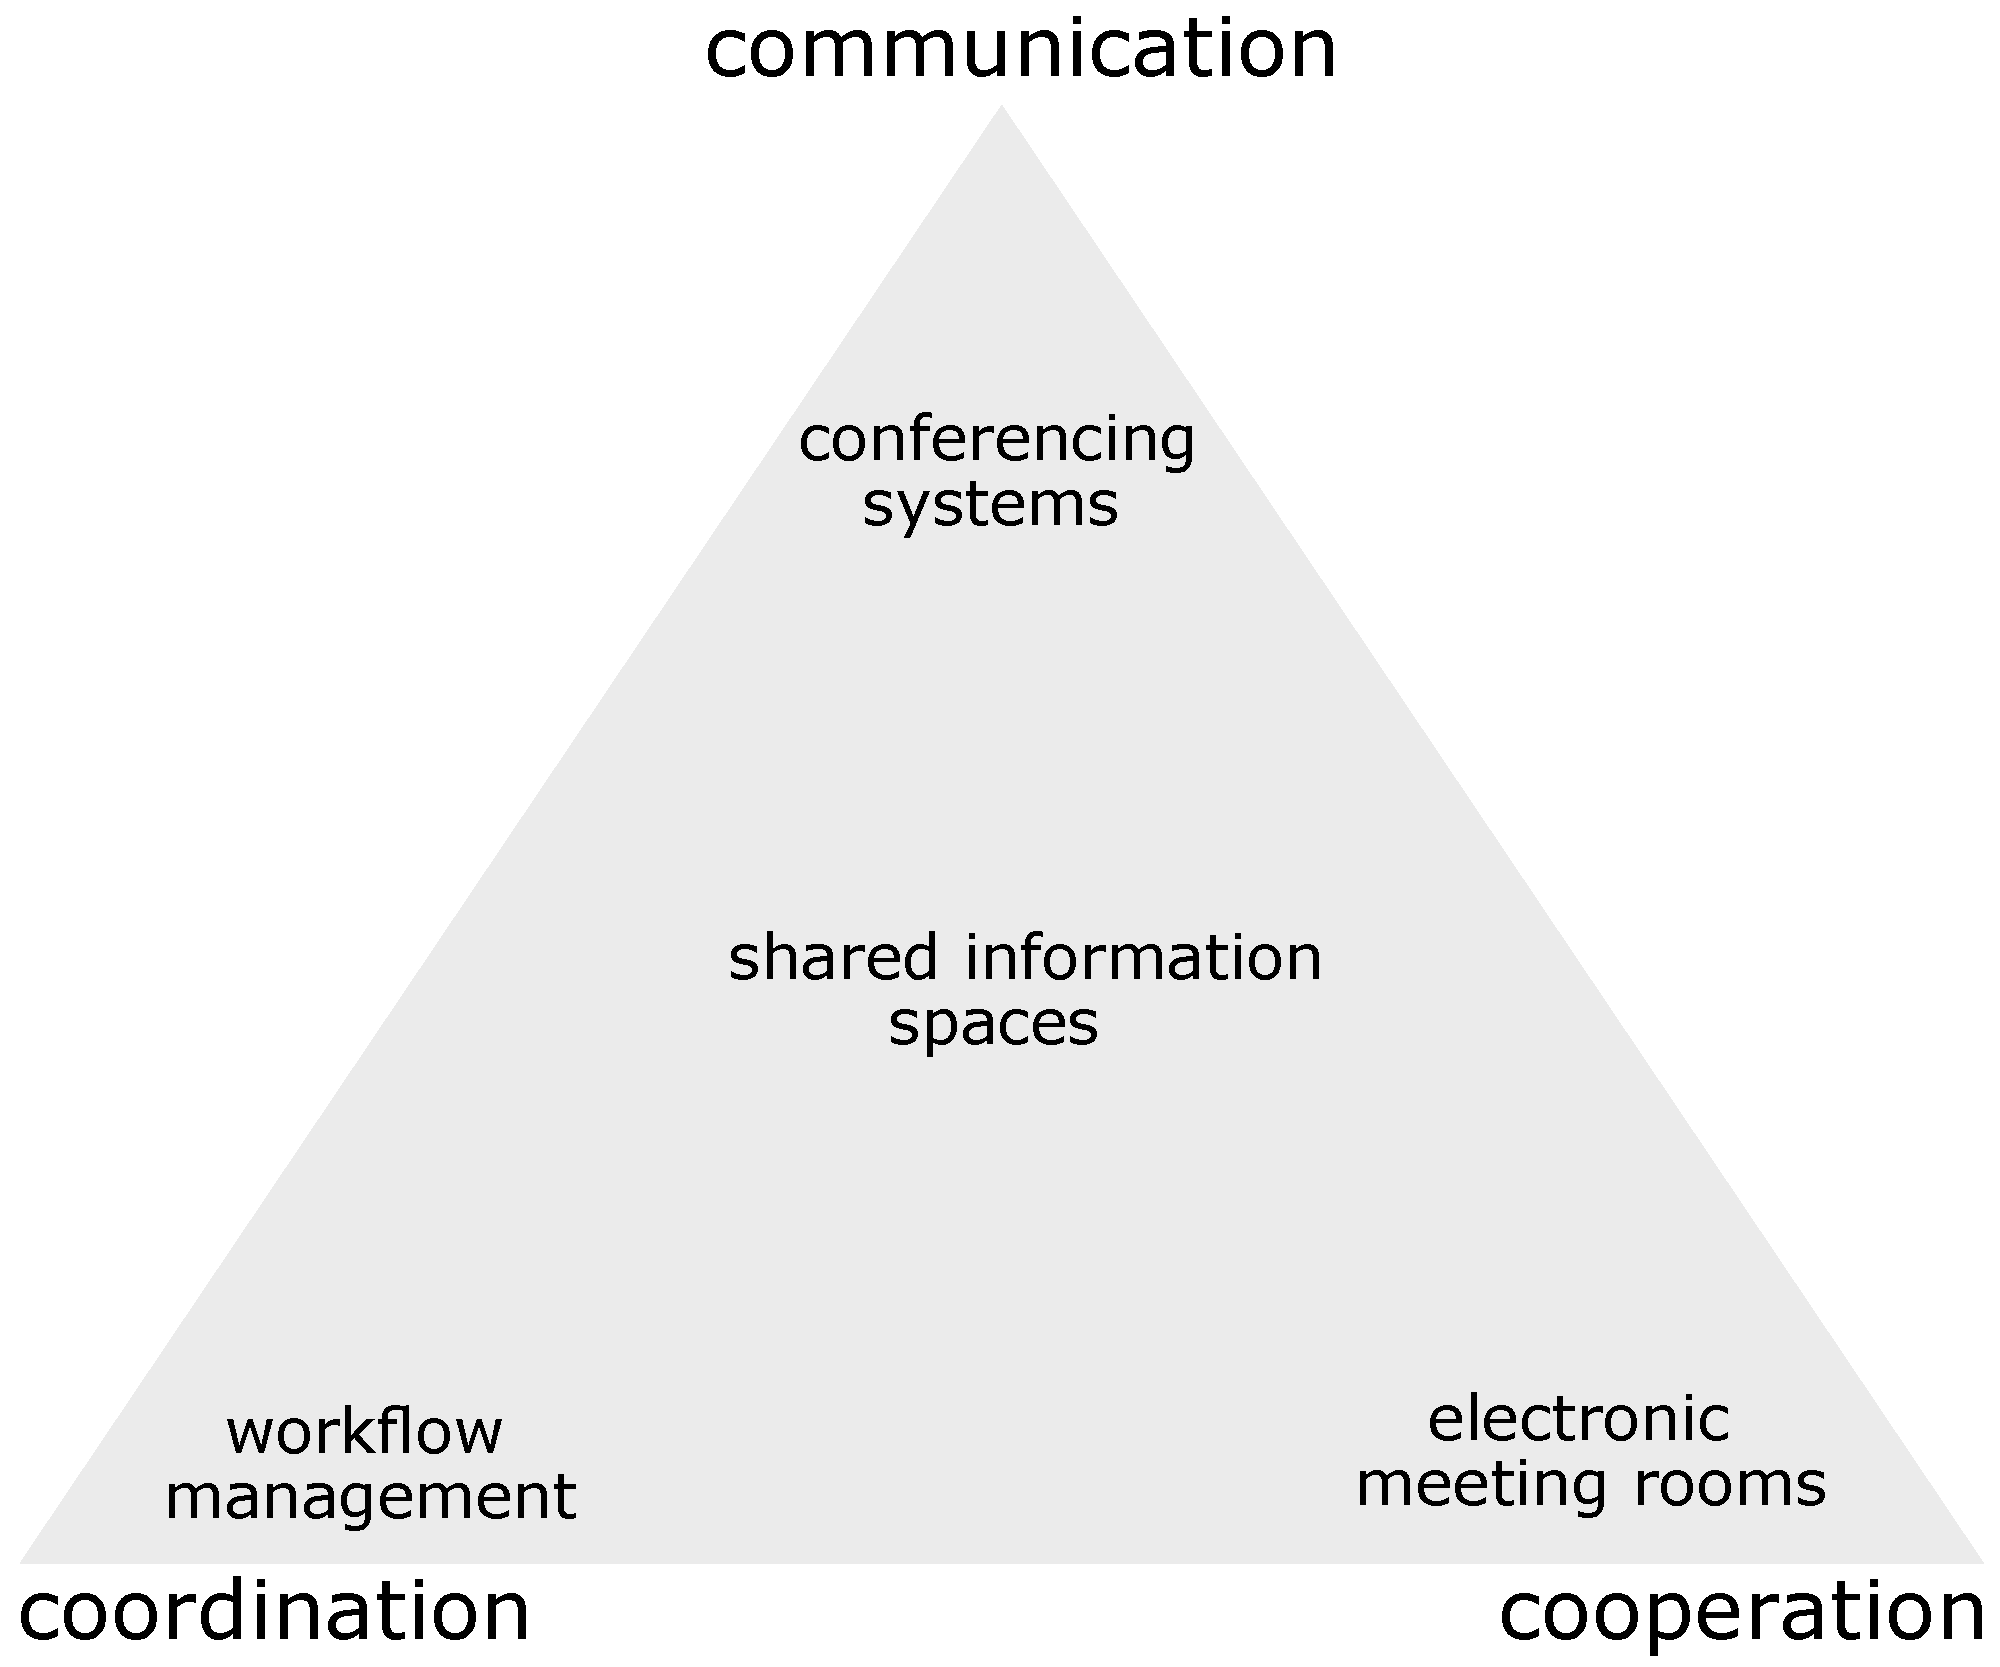
\includegraphics[width=0.8\columnwidth]{images/3C-model.pdf}
 \caption{The 3C Model \citep{Koch2008}}
\label{fig:images_cscw_3C_model}
\end{figure}

% section cscw_types (end)

\subsection{Shared Information Spaces}
\label{sec:cscw_shared_spaces}

% section cscw_shared_spaces (end)

\subsection{Important aspects of CSCW systems}
\label{sec:cscw_req_aspects}

% section cscw_req_aspects (end)

% section cscw (end)
